\section{Техническое задание}
\subsection{Основание для разработки}

Основанием для разработки является задание на выпускную квалификационную работу бакалавра "<Веб-приложение для компьютерной поддержки самостоятельной работы  иностранных студентов при изучении языка программирования  JavaScript">.

\subsection{Цель и назначение разработки}

Основной задачей выпускной квалификационной работы является разработка и внедрение веб-приложения для компьютерной поддержки самостоятельной работы  иностранных студентов при изучении языка программирования  JavaScript.

Посредством внедрения веб-приложения планируется устранить существующие недостатки, связанные с неструктурированным доступом к учебным материалам, отсутствием интерактивных инструментов для практики и тестирования, а также сложностями в организации учебного процесса для иностранных студентов, включая языковые барьеры.

Цель разработки включает следующие подцели:

\begin{itemize}
\item создание единой образовательной платформы для доступа к учебным курсам, урокам и тестам;
\item обеспечение удобного и интуитивно понятного интерфейса для самостоятельного изучения JavaScript;
\item интеграция инструментов для проверки знаний, таких как тесты с автоматической оценкой;
\item оптимизация процессов управления учебным контентом для преподавателей и взаимодействия студентов с платформой.
\end{itemize}

\subsection{Функциональные задачи}

Разрабатываемая веб-платформа включает в себя следующие модули:
\begin{enumerate}
\item {Курсы} — модуль для создания и управления учебными курсами, включающими уроки и тесты. Преподаватели могут добавлять, редактировать и удалять курсы, а студенты получают доступ к материалам.
\item {Уроки} — система управления учебным контентом, позволяющая структурировать материалы курса (текст, изображения, видео) и задавать порядок уроков. Поддерживается предпросмотр уроков и их редактирование.
\item {Тесты} — модуль для создания и прохождения интерактивных тестов. Преподаватели могут задавать вопросы и варианты ответов, а студенты проходят тесты с автоматической оценкой результатов.
\item {Результаты тестов} — инструмент для анализа успеваемости студентов. Преподаватели могут просматривать, удалять и управлять результатами тестов, включая статистику по студентам.
\item {Панель управления преподавателя} — интерфейс для управления курсами, уроками, тестами и результатами, с удобной навигацией и виджетами для быстрого доступа.
\item {Профиль пользователя} — модуль для управления учетной записью, включая настройки аватара и персональной информации.
\item {Сообщения} — система уведомлений для обратной связи (например, сообщения об успешном добавлении урока или удалении результатов).
\item {Панель управления} — страница с виджетами всех вышеперечисленных сервисов.
\end{enumerate}

\subsection{Требования пользователя к интерфейсу web-сайта}

Платформа должна обеспечивать:
\begin{itemize}
    \item авторизацию;
    \item интуитивно понятную навигацию между модулями;
    \item адаптивный интерфейс для десктопных и мобильных устройств.
\end{itemize}

Композиция интерфейса пользователя представлена на рисунках ~\ref{templ:image1}, ~\ref{templ:image2}, ~\ref{templ:image3}, ~\ref{templ:image4}, ~\ref{templ:image5}, ~\ref{templ:image6}, ~\ref{templ:image7}, ~\ref{templ:image8}, ~\ref{templ:image9},  ~\ref{templ:image10}.
\newpage  

Композиция шаблона курсы представлена на рисунке ~\ref{templ:image1} и состоит из:

\begin{itemize}
	\item кнопка для просмотра курса (1);
	\item окна с информацией роли профиля и имени (2);
	\item кнопка для создания курса (3);
	\item кнопка для просмотра своих курсов (4);
	\item кнопка для выхода (5);
	\item кнопка для смены языка (6).
\end{itemize}

\begin{figure}[h]
	\centering
	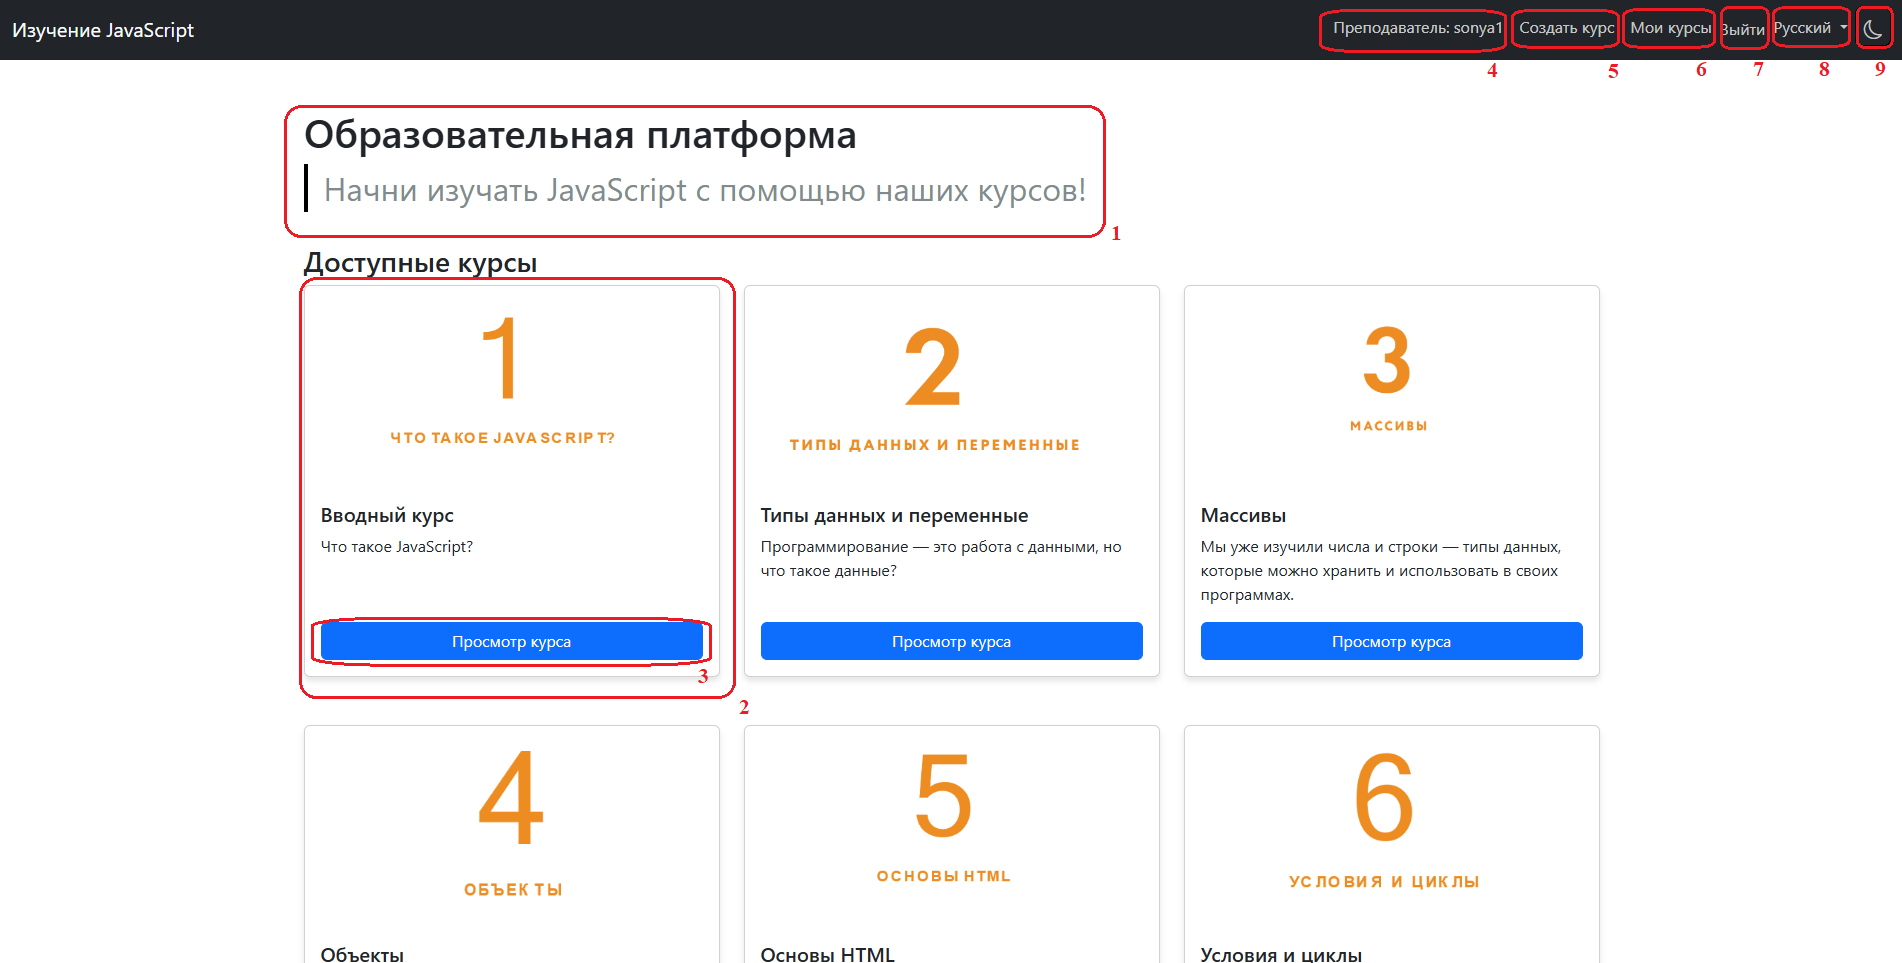
\includegraphics[width=1\linewidth]{images/курсы}
	\caption{Композиция интерфейса сервиса <<Курсы>>}
	\label{templ:image1}
\end{figure}

Композиция шаблона панель управления преподавателя представлена на рисунке ~\ref{templ:image2} и состоит из:

\begin{itemize}
	\item кнопка для редактирования курса (1);
	\item кнопка для управления уроками (2);
	\item кнопка для просмотра курса (3);
	\item кнопка для удаления курса (4).
\end{itemize}

\begin{figure}[h]
	\centering
	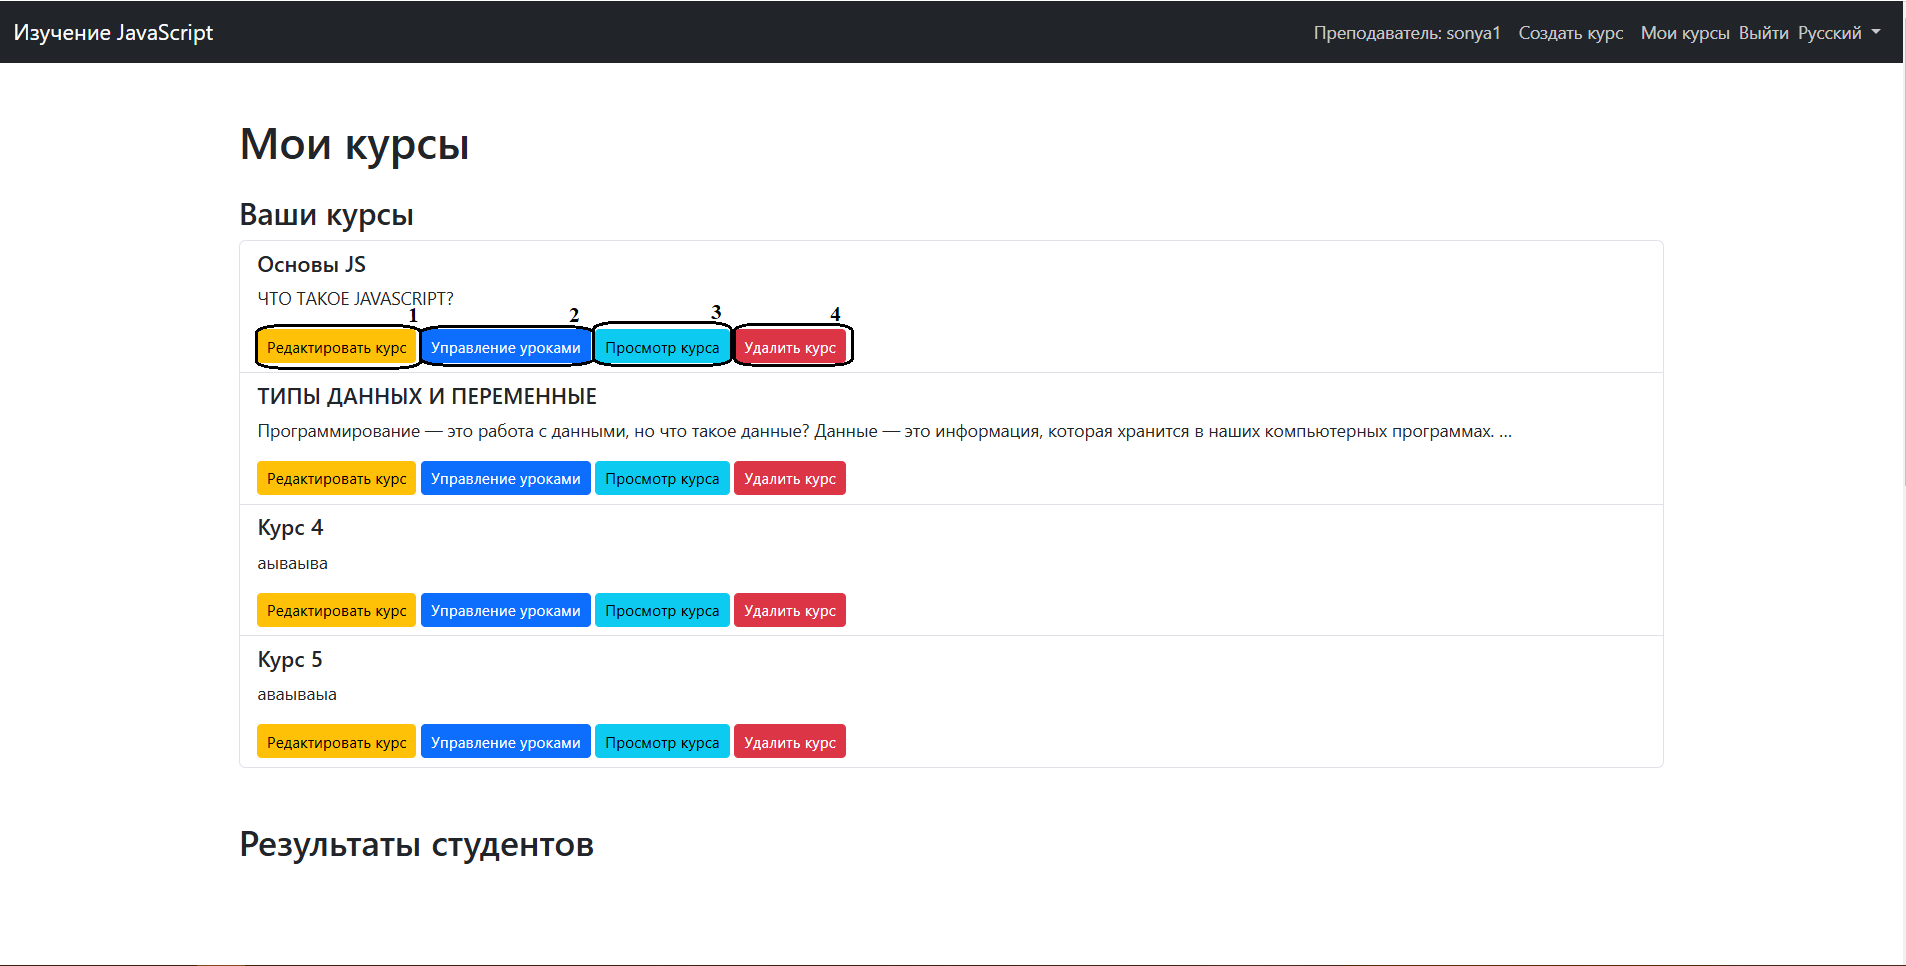
\includegraphics[width=1\linewidth]{images/учитель}
	\caption{Композиция интерфейса сервиса <<Панель управления преподавателя>>}
	\label{templ:image2}
\end{figure}
\newpage 

Композиция шаблона уроки представлена на рисунке ~\ref{templ:image3} и состоит из:

\begin{itemize}
	\item кнопка для просмотра урока (1);
	\item окна курса (2);
	\item окно уроков (3);
	\item навигационная панель (4).
\end{itemize}

\begin{figure}[h]
	\centering
	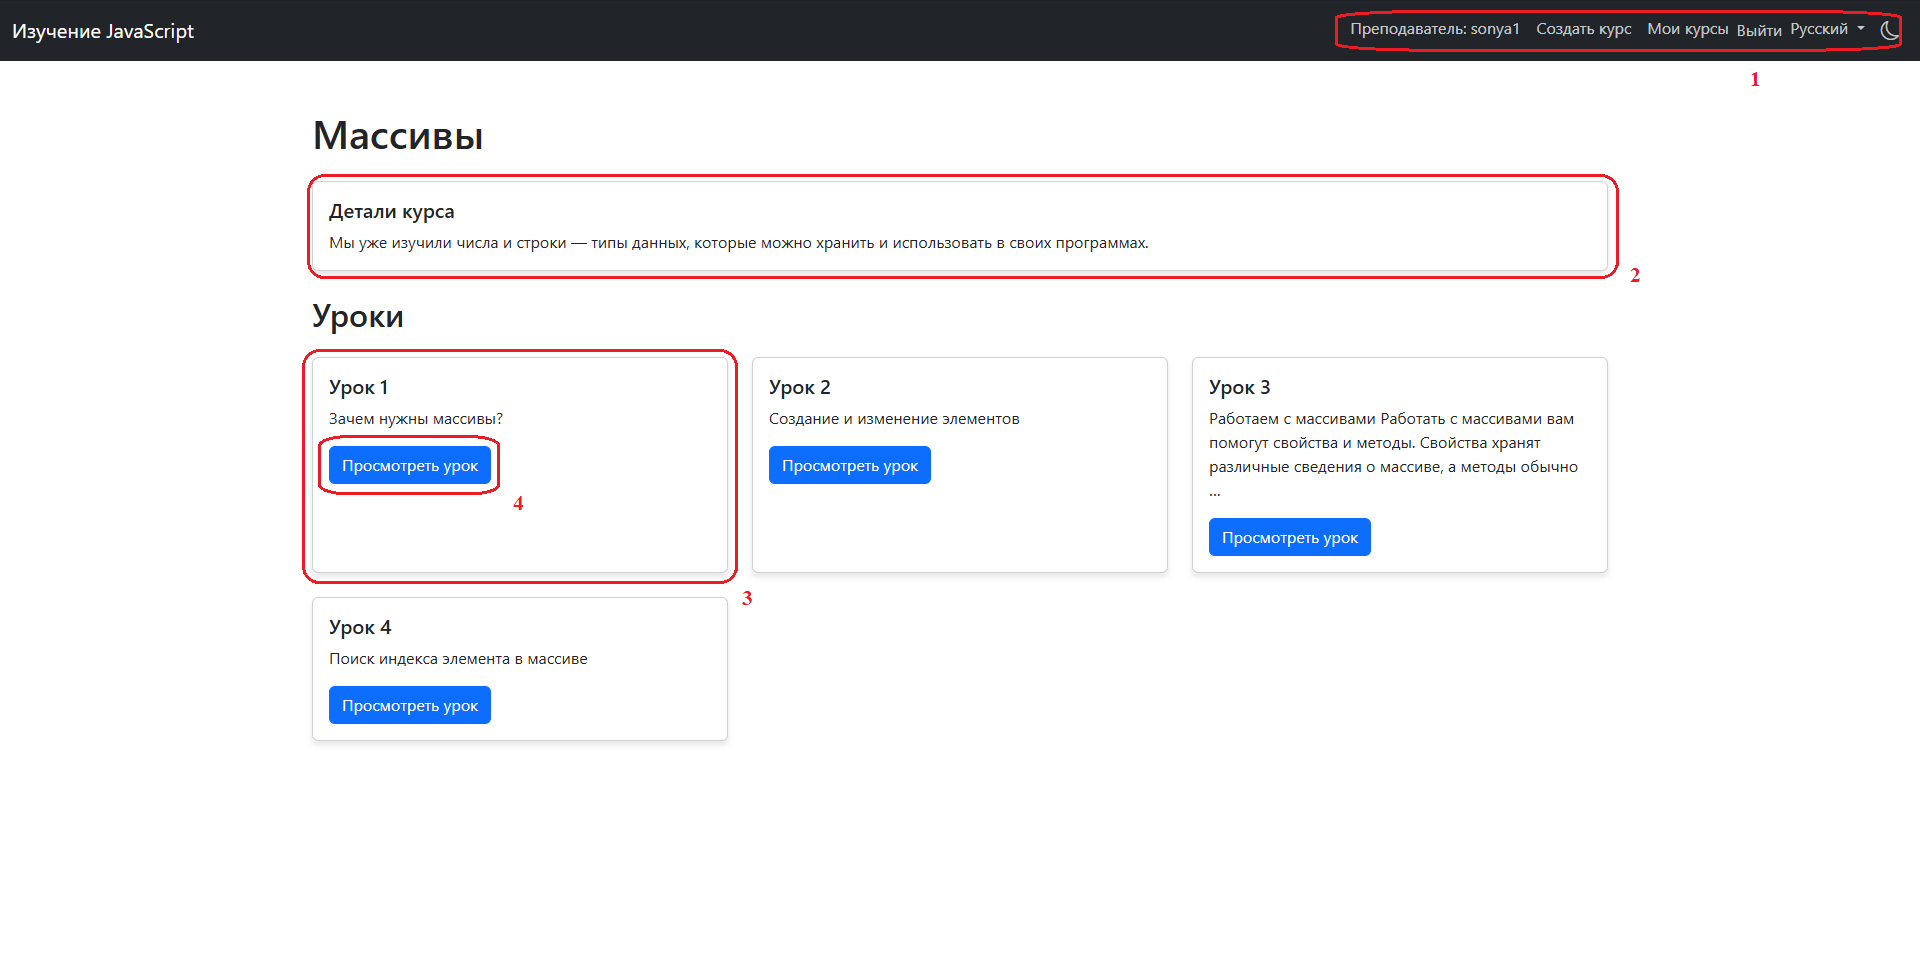
\includegraphics[width=1\linewidth]{images/уроки}
	\caption{Композиция интерфейса сервиса <<Уроки>>}
	\label{templ:image3}
\end{figure}

Композиция шаблона тесты представлена на рисунке ~\ref{templ:image4} и состоит из:

\begin{itemize}
	\item окно уроков (1);
	\item кнопка редактировать урок (2);
	\item кнопка просмотр урока (3);
	\item кнопка обложка урока (4);
	\item кнопка добавить тест (5);
	\item кнопка управление вопросами (6);
	\item кнопка управление результатами (7).
\end{itemize}

\begin{figure}[h]
	\centering
	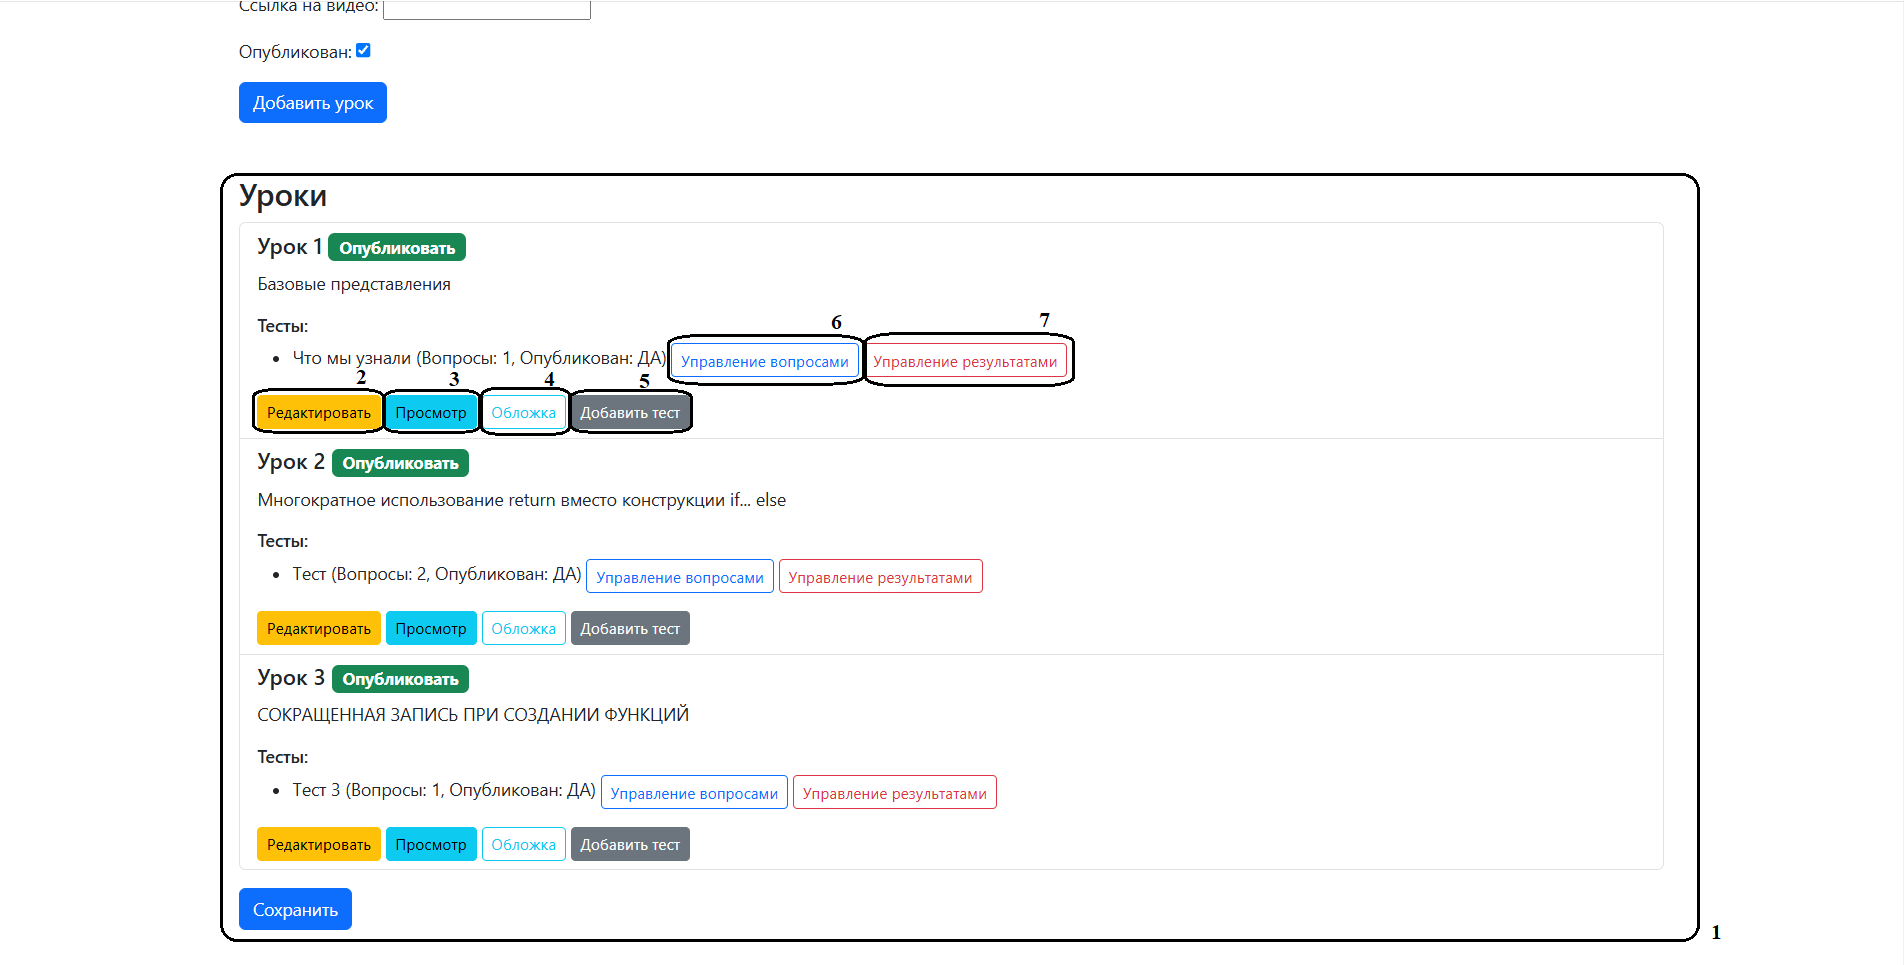
\includegraphics[width=1\linewidth]{images/Тесты}
	\caption{Композиция интерфейса сервиса <<Тесты>>}
	\label{templ:image4}
\end{figure}

Композиция шаблона создание теста представлена на рисунке ~\ref{templ:image5} и состоит из:

\begin{itemize}
	\item окно создания теста (1);
	\item поле ввода заголовка теста (2);
	\item поле ввода описания теста (3);
	\item поле ввода минимального балла (4);
	\item поле выбора статуса (5);
	\item кнопка для создания теста (6);
	\item кнопка возвращения к уроку (7).
\end{itemize}

\begin{figure}[h]
	\centering
	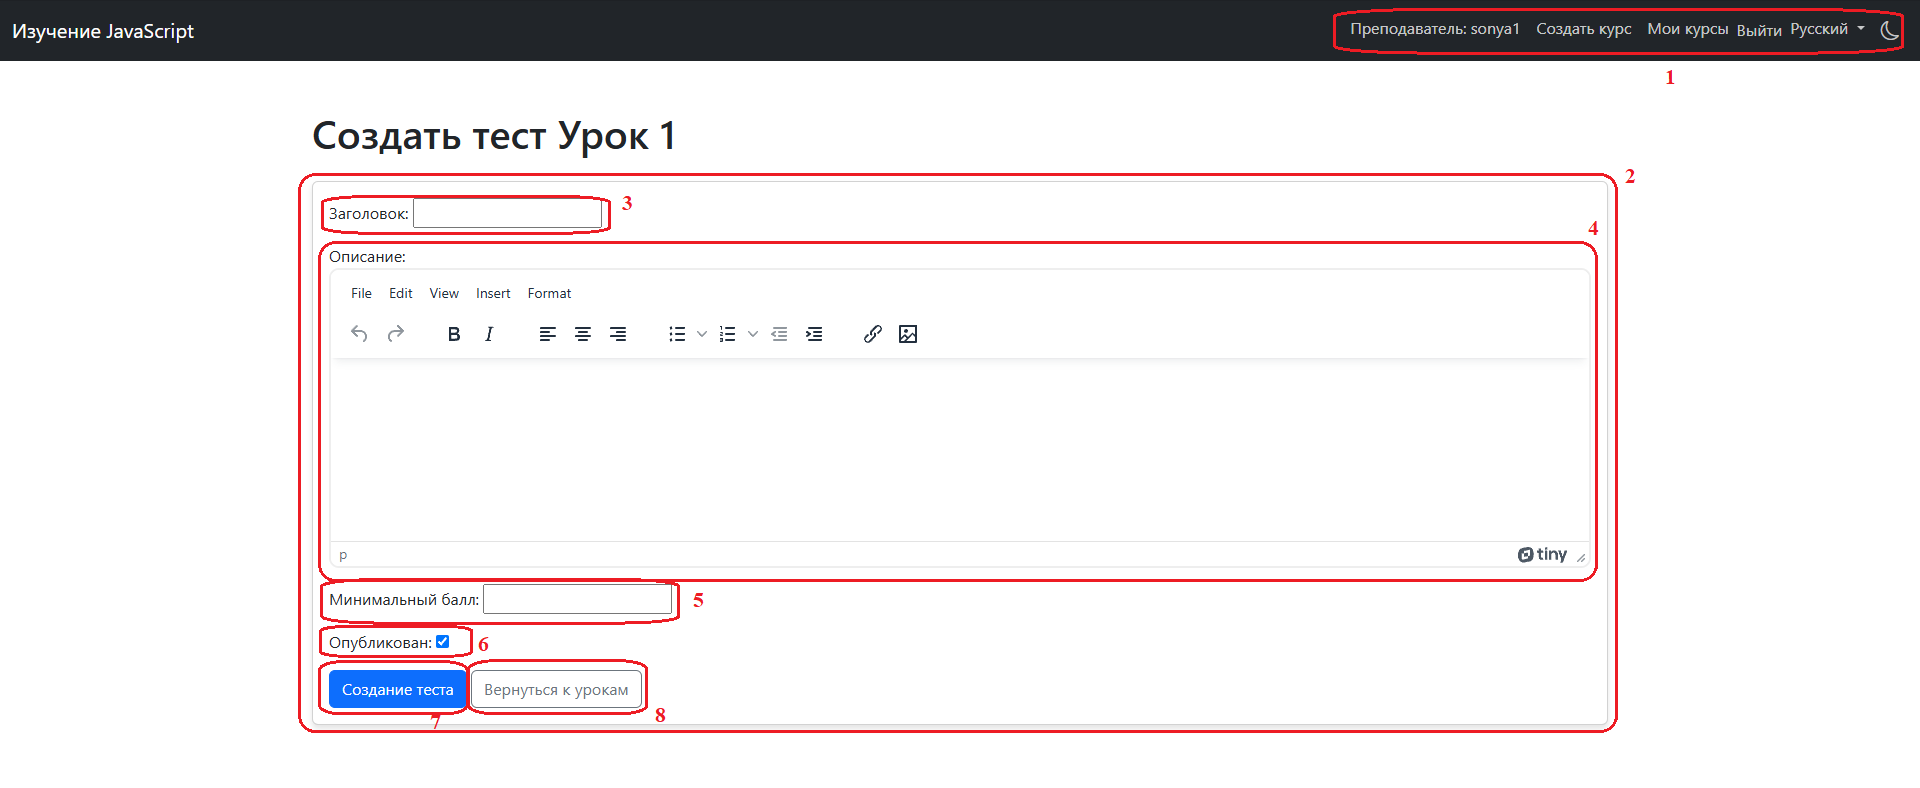
\includegraphics[width=1\linewidth]{images/создатьтест}
	\caption{Композиция интерфейса сервиса <<Создание теста>>}
	\label{templ:image5}
\end{figure}
\newpage

Композиция шаблона результаты теста представлена на рисунке ~\ref{templ:image6} и состоит из:

\begin{itemize}
	\item окна управления результатами теста (1);
	\item окна с результатами студентов  (2);
	\item кнопка удалить все результаты (3);
	\item кнопка удалить результат (4);
	\item кнопка вернуться к вопросам (5);
	\item кнопка вернуться к урокам (6).
\end{itemize}

\begin{figure}[h]
	\centering
	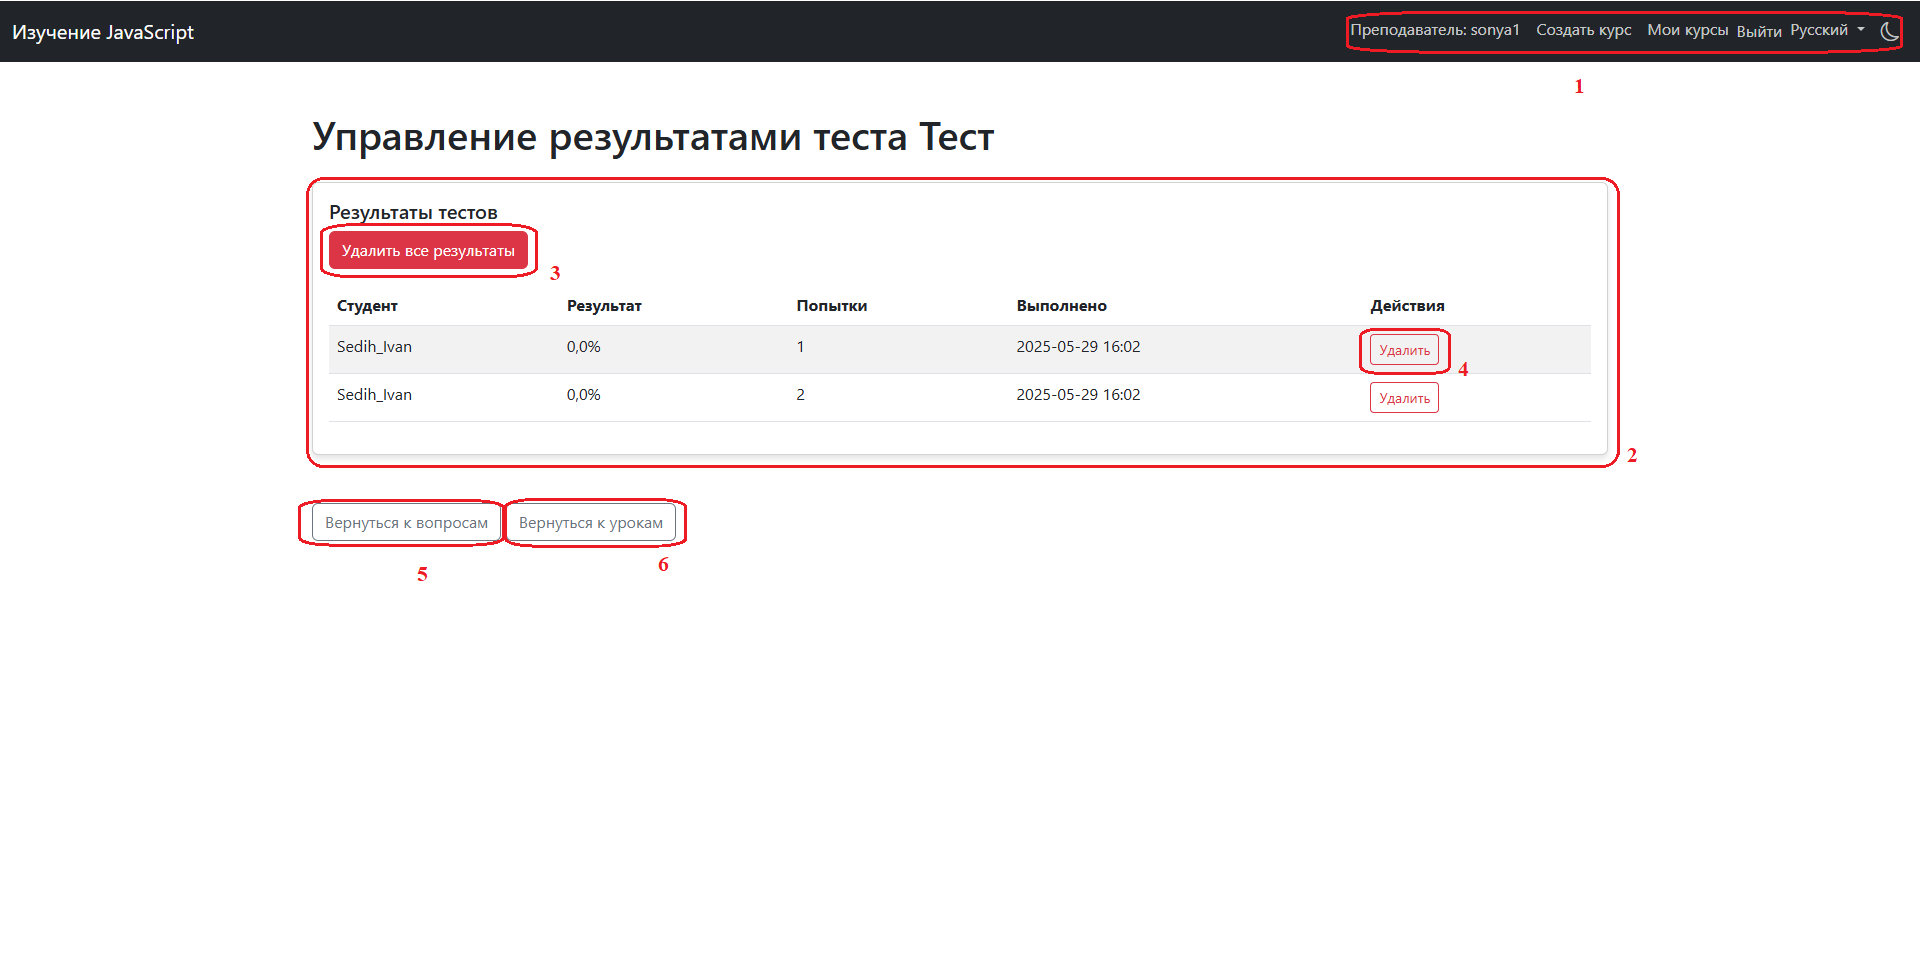
\includegraphics[width=1\linewidth]{images/результаты}
	\caption{Композиция интерфейса сервиса <<Результаты тестов>>}
	\label{templ:image6}
\end{figure}
\newpage
Композиция шаблона окна авторизации представлена на рисунке ~\ref{templ:image7} и состоит из:

\begin{itemize}
	\item поле для ввода кода (1);
	\item экранная клавиатура (2);
	\item кнопка для очистки поля (3);
	\item кнопка для подтверждения ввода пароля (4).
\end{itemize}

\begin{figure}[h]
	\centering
	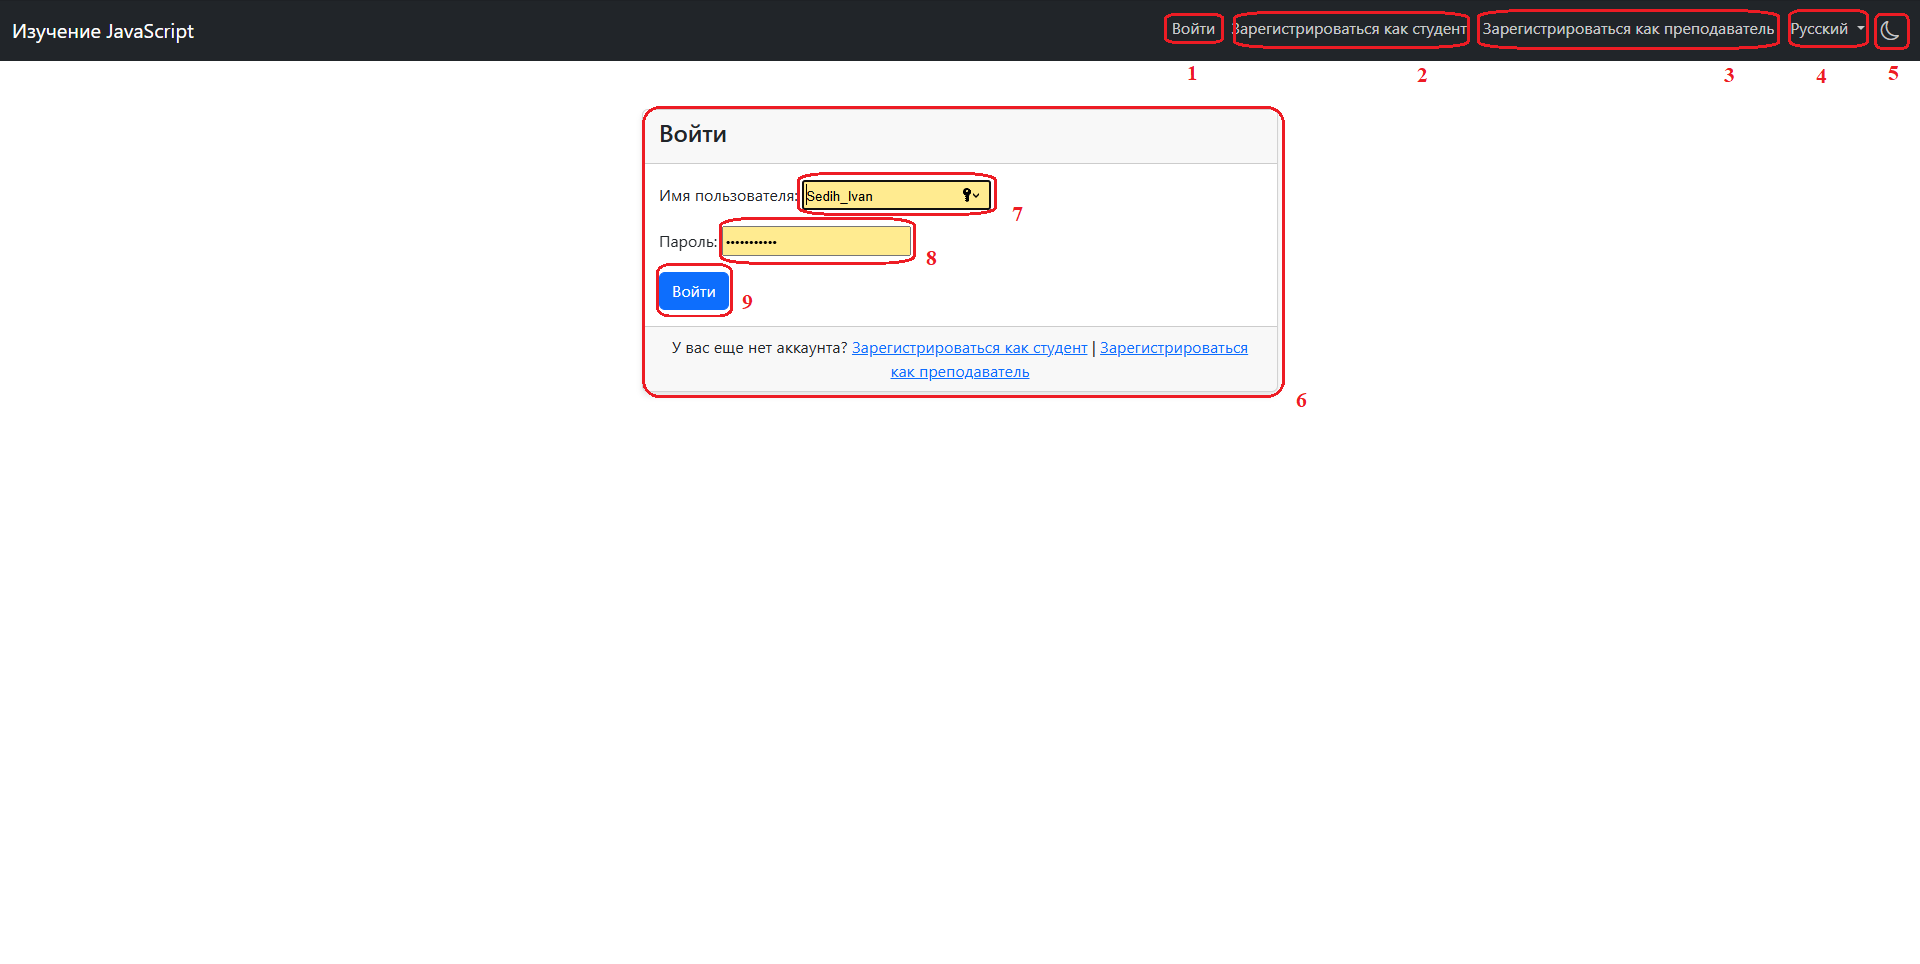
\includegraphics[width=1\linewidth]{images/Авторизация}
	\caption{Композиция интерфейса сервиса <<Авторизация>>}
	\label{templ:image7}
\end{figure}

Композиция шаблона профиль представлена на рисунке ~\ref{templ:image8} и состоит из:

\begin{itemize}
	\item окно курсов на которые записан (1);
	\item кнопка просмотра курса (2);
	\item кнопка отписаться (3).
\end{itemize}

\begin{figure}[h]
	\centering
	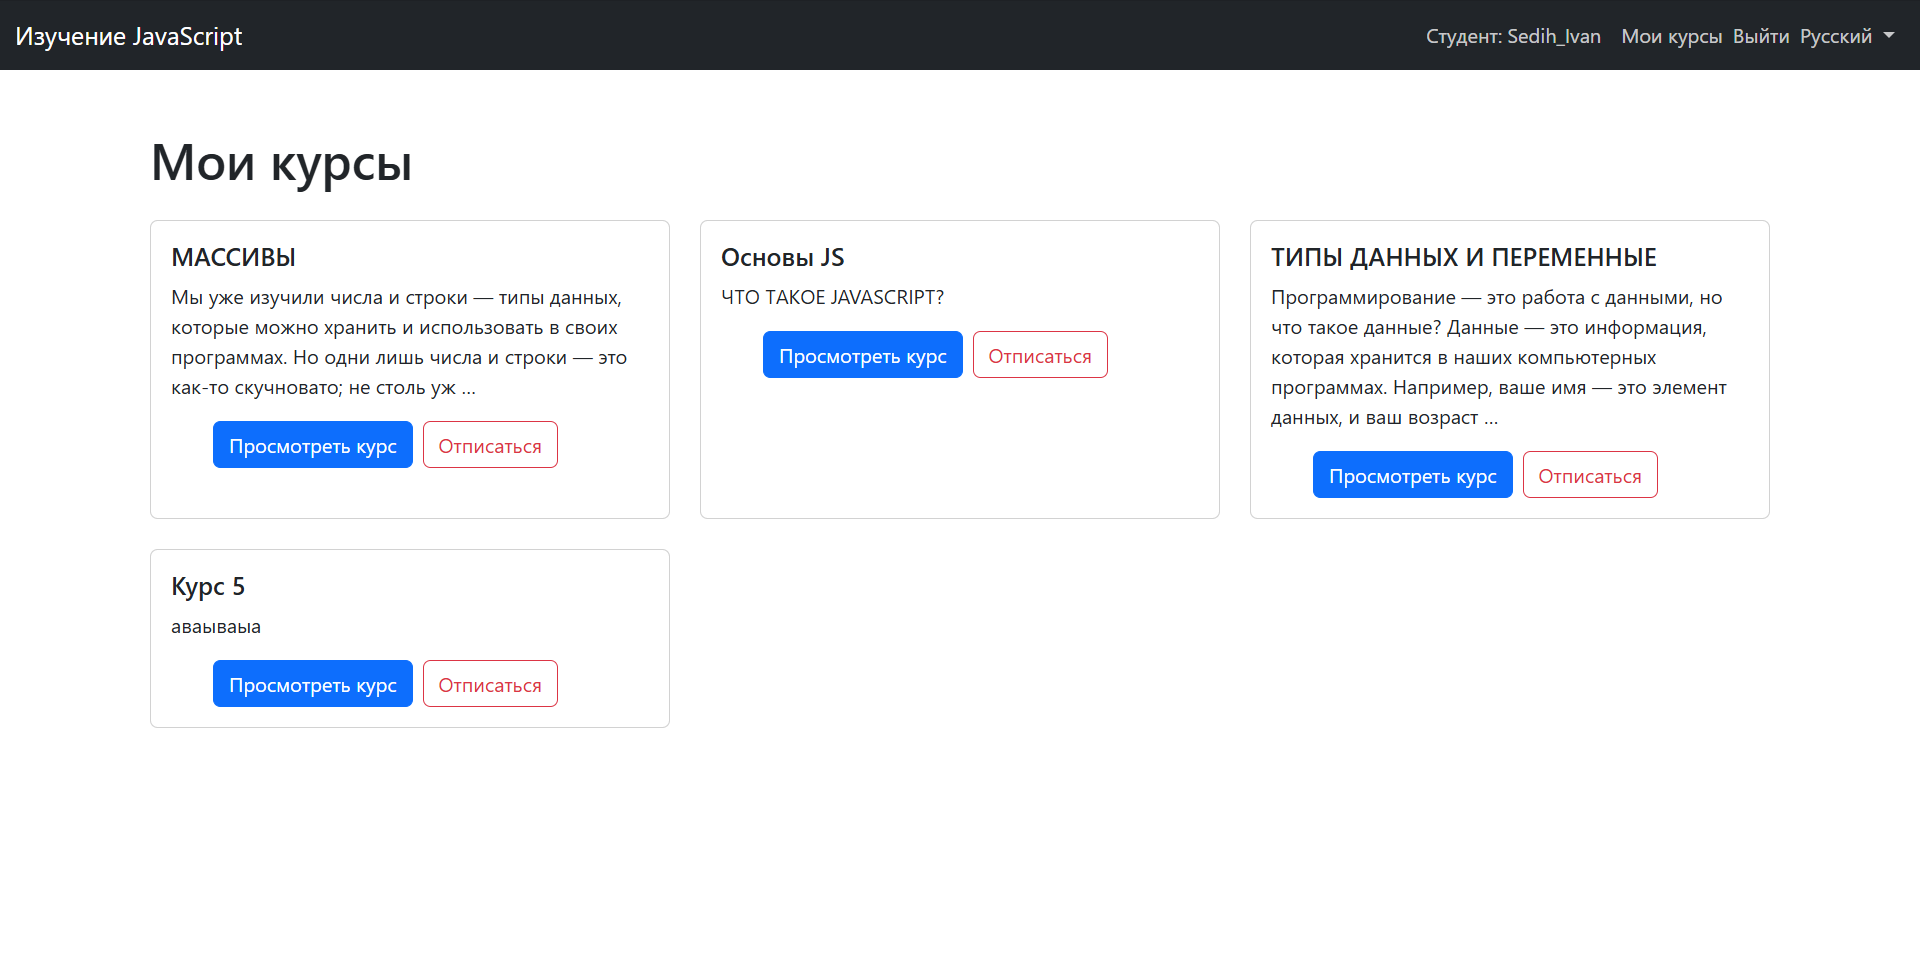
\includegraphics[width=1\linewidth]{images/профиль}
	\caption{Композиция интерфейса сервиса <<Профиль>>}
	\label{templ:image8}
\end{figure}


Композиция шаблона создание курса представлена на рисунке ~\ref{templ:image9} и состоит из:

\begin{itemize}
	\item окно создания курса (1);
	\item поле ввода заголовка курса (2);
	\item поле ввода описания курса (3);
	\item кнопка выбора изображения (4);
	\item поле выбора статуса курса (5);
	\item кнопка сохранения курса (6);
	\item кнопка отмены создания курса (7).
\end{itemize}

\begin{figure}[h]
	\centering
	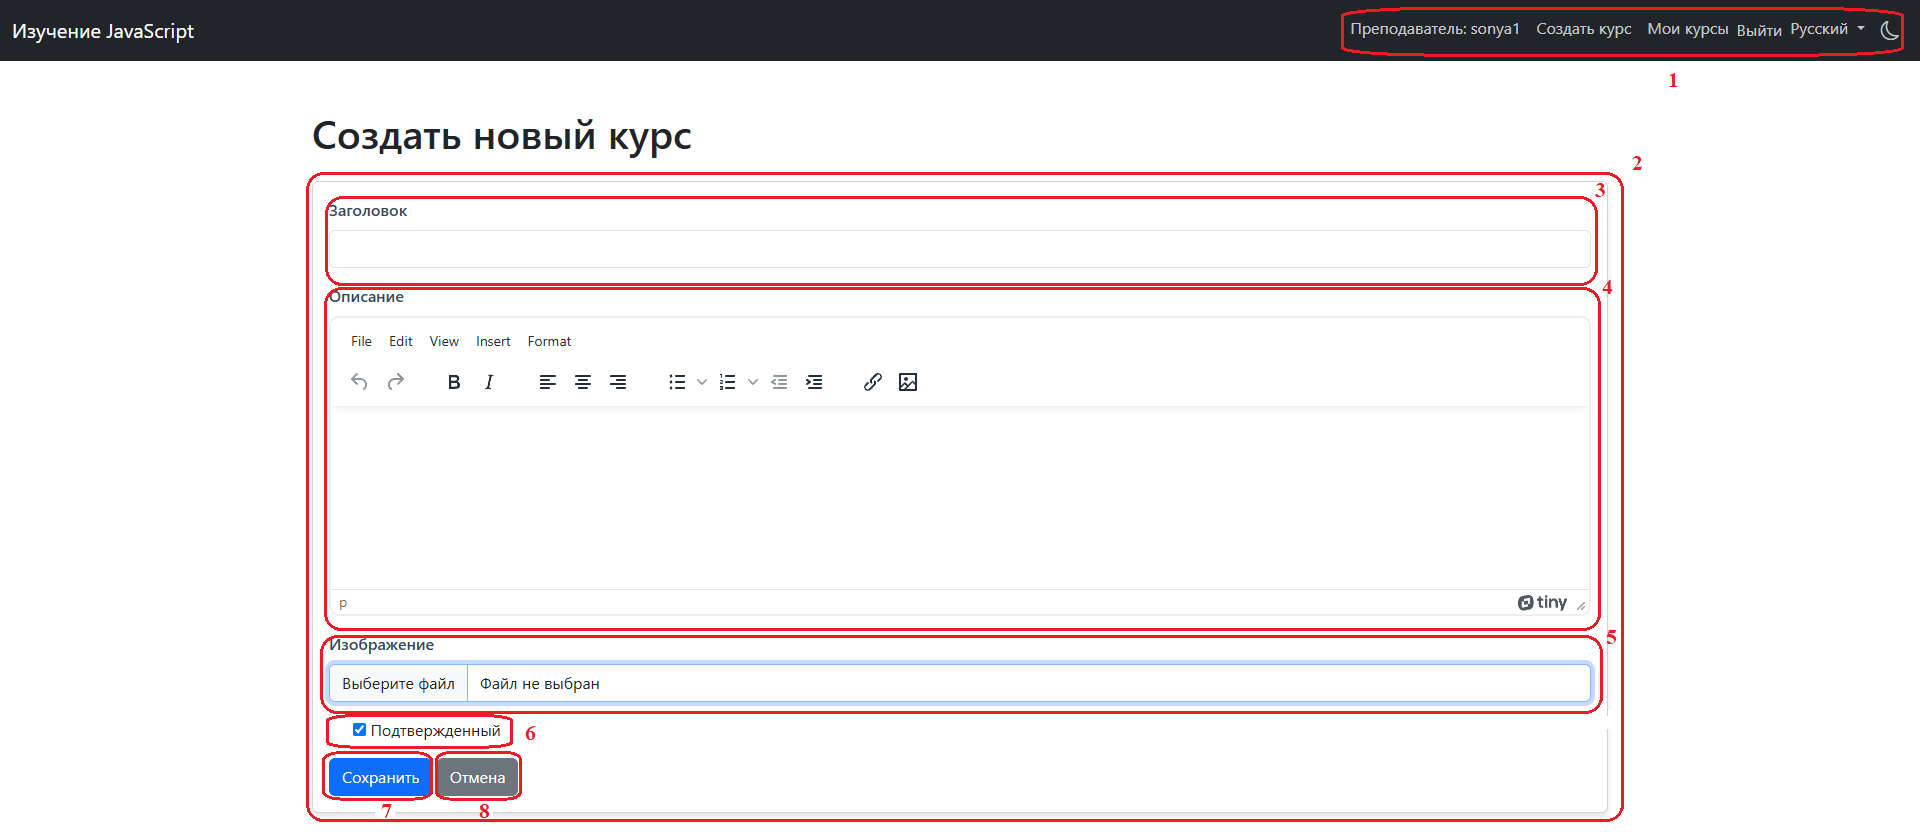
\includegraphics[width=0.9\linewidth]{images/создатькурс}
	\caption{Композиция интерфейса сервиса <<Создание курса>>}
	\label{templ:image9}
\end{figure}

\newpage
Композиция шаблона создание урока представлена на рисунке ~\ref{templ:image10} и состоит из:

\begin{itemize}
	\item окно создания урока (1);
	\item поле ввода заголовка урока (2);
	\item поле ввода описания урока (3);
	\item поле ввода материалов урока (4);
	\item поле ввода ссылки на видеоролик (5);
	\item поле выбора статуса урока (6);
	\item кнопка добавления урока (7).
\end{itemize}

\begin{figure}[h]
	\centering
	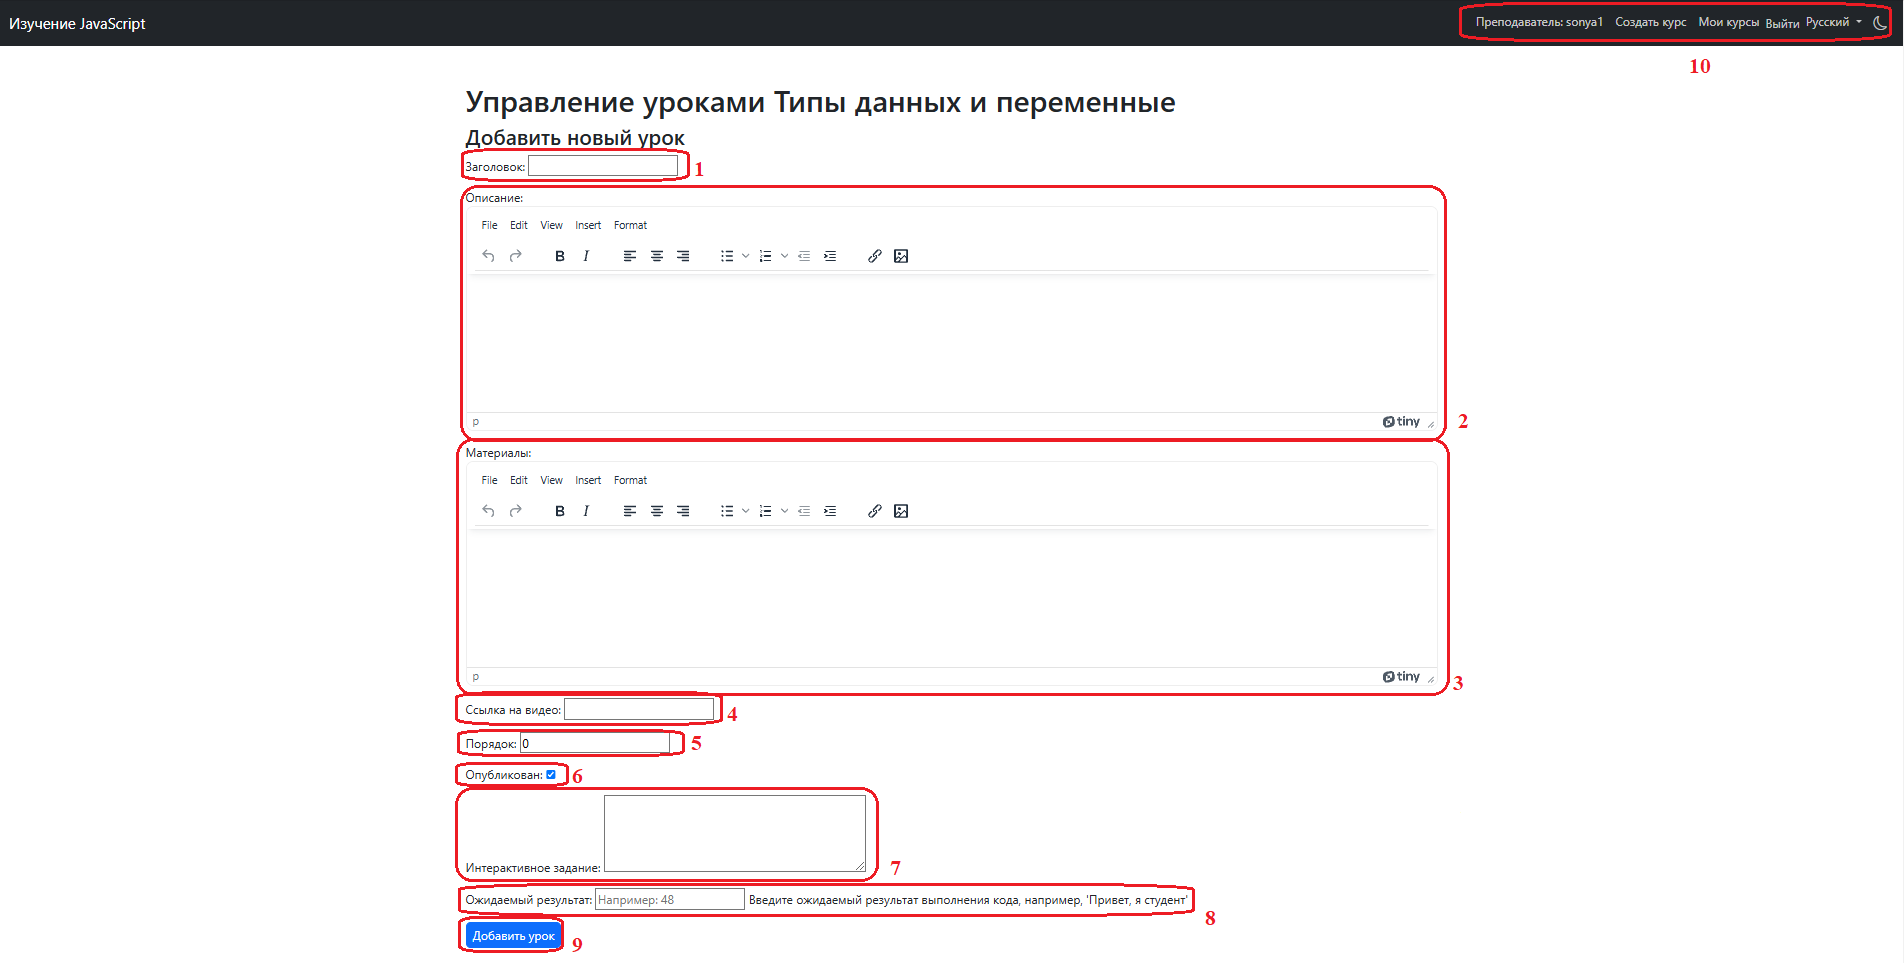
\includegraphics[width=0.9\linewidth]{images/создатьурок}
	\caption{Композиция интерфейса сервиса <<Создание урока>>}
	\label{templ:image10}
\end{figure}

\clearpage
\subsection{Моделирование вариантов использования}

Для разработки платформы была построена UML-диаграмма вариантов использования, отражающая взаимодействие пользователей с системой.

\begin{figure}[ht]
	\center{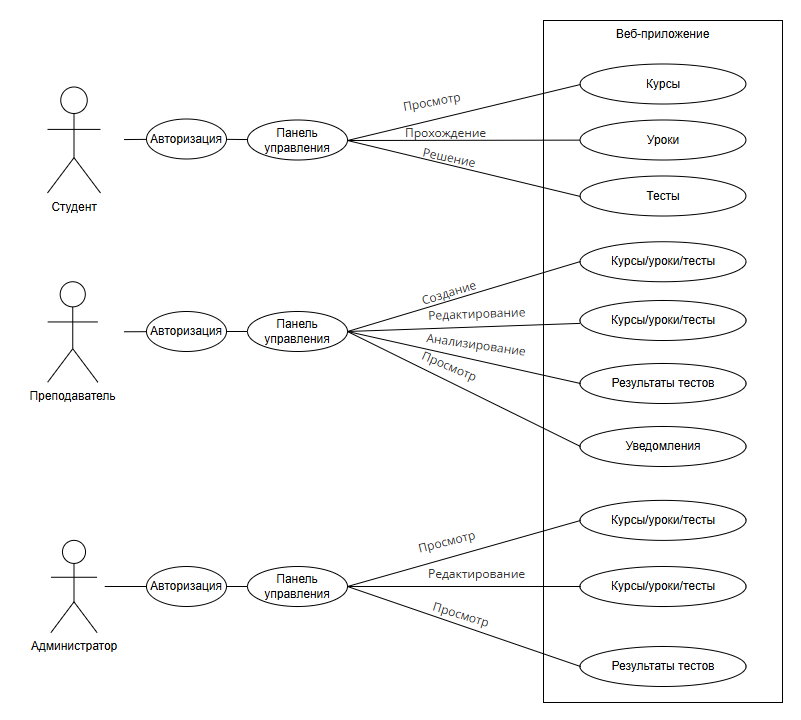
\includegraphics[width=1\linewidth]{images/UML}}
	\caption{Диаграмма прецедентов}
	\label{comp:image}
\end{figure}

Основные прецеденты системы:

\begin{enumerate}
	\item {Авторизация и выход из системы}: Позволяет пользователям (преподавателям, студентам, администраторам) входить в систему и выходить из неё.
	\item {Управление курсами}: Обеспечивает создание, редактирование и удаление курсов преподавателями, а также просмотр и запись на курсы студентами.
	\item {Управление уроками}: Дает возможность преподавателям управлять уроками, а студентам --- изучать их материалы.
	\item {Создание и управление тестами}: Позволяет преподавателям создавать тесты, а студентам --- проходить их.
	\item {Прохождение тестов}: Обеспечивает студентам возможность проходить тесты с автоматической оценкой.
	\item {Просмотр результатов тестов}: Позволяет преподавателям и студентам анализировать результаты.
	\item {Локализация интерфейса}: Обеспечивает переключение языка интерфейса для удобства пользователей.
\end{enumerate}

После авторизации пользователь переходит на главную страницу: преподаватели видят панель управления, студенты --- список доступных курсов. Ниже приведено подробное описание каждого сервиса и связанных прецедентов.

\begin{enumerate}
	\item {Сервис <<Курсы>>}
	
	{Прецедент: Управление курсами (для преподавателей)} \\
	{Цель}: Создание, редактирование и удаление курсов. \\
	{Актёр}: Преподаватель. \\
	{Предусловие}: Преподаватель авторизован и находится в панели управления. \\
	{Основной сценарий}:
	\begin{itemize}
		\item преподаватель переходит в раздел <<Курсы>>;
		\item нажимает кнопку <<Создать курс>>;
		\item заполняет форму: название (title), описание (description), изображение (image), статус активности (isactive);
		\item сохраняет курс, система добавляет его в базу данных (courses\_course) и связывает с преподавателем (teacherid);
		\item для редактирования или удаления преподаватель выбирает курс из списка и выполняет соответствующее действие.
	\end{itemize}
	{Постусловие}: Курс создан, отредактирован или удалён, изменения отражены в базе данных. \\
	{Альтернативный сценарий}: Если форма заполнена некорректно (например, пустое название), система выдаёт уведомление об ошибке.
	
	{Прецедент: Просмотр и запись на курсы (для студентов)} \\
	{Цель}: Просмотр доступных курсов и запись на них. \\
	{Актёр}: Студент. \\
	{Предусловие}: Студент авторизован. \\
	{Основной сценарий}:
	\begin{itemize}
		\item студент переходит на главную страницу, где отображается список курсов;
		\item список включает название, описание и статус курса (например, <<Доступен>>, <<Завершён>>);
		\item студент выбирает курс и нажимает кнопку <<Записаться>>;
		\item система добавляет запись в таблицу <<Запись на курсы>> (courses\_enrollment) с полями (courseid), (studentid), (enrolledat).
	\end{itemize}
	{Постусловие}: Студент записан на курс, запись отражена в базе данных.
	
	\item {Сервис <<Уроки>>}
	
	{Прецедент: Управление уроками (для преподавателей)} \\
	{Цель}: Добавление, редактирование, сортировка и удаление уроков в рамках курса. \\
	{Актёр}: Преподаватель. \\
	{Предусловие}: Преподаватель авторизован, выбран курс. \\
	{Основной сценарий}:
	\begin{itemize}
		\item преподаватель переходит в раздел <<Уроки>> выбранного курса;
		\item нажимает кнопку <<Добавить урок>>;
		\item заполняет форму: название (title), описание (description), содержимое (content), ссылка на видео (videourl), порядок (order), статус публикации (ispublished);
		\item сохраняет урок, система добавляет его в таблицу (courses\_lesson);
		\item для сортировки использует интерфейс с Sortable.js, изменяя поле (order);
		\item для редактирования или удаления выбирает урок из списка;
		\item может включить предпросмотр урока перед публикацией.
	\end{itemize}
	{Постусловие}: Урок добавлен, отредактирован, отсортирован или удалён. \\
	{Альтернативный сценарий}: Если видео-URL недействителен, система уведомляет об ошибке.
	
	{Прецедент: Изучение уроков (для студентов)} \\
	{Цель}: Просмотр материалов урока. \\
	{Актёр}: Студент. \\
	{Предусловие}: Студент записан на курс, урок опубликован. \\
	{Основной сценарий}:
	\begin{itemize}
		\item студент выбирает курс и переходит в раздел <<Уроки>>;
		\item видит список уроков, отсортированных по полю (order);
		\item выбирает урок и просматривает материалы: текст (content), видео (videourl);
		\item после завершения урока система обновляет прогресс (courses\_progress): (completed).
	\end{itemize}
	{Постусловие}: Урок изучен, прогресс обновлён.
	
	\item {Сервис <<Тесты>>}
	
	{Прецедент: Создание и управление тестами (для преподавателей)} \\
	{Цель}: Создание тестов с вопросами и ответами. \\
	{Актёр}: Преподаватель. \\
	{Предусловие}: Преподаватель авторизован, выбран урок. \\
	{Основной сценарий}:
	\begin{itemize}
		\item преподаватель переходит в раздел <<Тесты>> урока;
		\item нажимает кнопку <<Создать тест>>;
		\item заполняет форму: название (title), описание (description), проходной балл (passingscore), статус (isactive);
		\item добавляет вопросы (courses\_question): текст (text), тип (questiontype), баллы (points);
		\item для каждого вопроса добавляет варианты ответа (courses\_answer): текст (text), правильность (iscorrect), порядок (order);
		\item сохраняет тест, система добавляет его в таблицу (courses\_test).
	\end{itemize}
	{Постусловие}: Тест создан и связан с уроком (lessonid). \\
	{Альтернативный сценарий}: Если проходной балл некорректен, система выдаёт ошибку.
	
	{Прецедент: Прохождение тестов (для студентов)} \\
	{Цель}: Прохождение теста и получение оценки. \\
	{Актёр}: Студент. \\
	{Предусловие}: Студент записан на курс, тест активен. \\
	{Основной сценарий}:
	\begin{itemize}
		\item студент переходит к уроку и выбирает тест;
		\item система отображает вопросы с вариантами ответов;
		\item студент выбирает ответы и отправляет тест;
		\item система автоматически оценивает ответы, сравнивая с (iscorrect), и сохраняет результат (courses\_testresult: score, answers, attempts).
	\end{itemize}
	{Постусловие}: Тест пройден, результат сохранён.
	
	\item {Сервис <<Результаты тестов>>}
	
	{Прецедент: Просмотр и анализ результатов (для преподавателей)} \\
	{Цель}: Анализ успеваемости студентов. \\
	{Актёр}: Преподаватель. \\
	{Предусловие}: Преподаватель авторизован, тест пройден хотя бы одним студентом. \\
	{Основной сценарий}:
	\begin{itemize}
		\item преподаватель переходит в раздел <<Результаты тестов>>;
		\item система отображает список студентов, их баллы (score), количество попыток (attempts) и ответы (answers);
		\item преподаватель может удалить результат, если он некорректен.
	\end{itemize}
	{Постусловие}: Преподаватель получил статистику по тесту. \\
	{Альтернативный сценарий}: Если результатов нет, отображается сообщение <<Нет данных>>.
	
	{Прецедент: Просмотр результатов (для студентов)} \\
	{Цель}: Просмотр своих баллов и статистики. \\
	{Актёр}: Студент. \\
	{Предусловие}: Студент прошёл тест. \\
	{Основной сценарий}:
	\begin{itemize}
		\item студент переходит в раздел <<Результаты>>;
		\item система отображает баллы (score), количество попыток (attempts) и правильные/неправильные ответы.
	\end{itemize}
	{Постусловие}: Студент увидел свои результаты.
	
	\item {Сервис <<Локализация>>}
	
	{Прецедент: Локализация интерфейса} \\
	{Цель}: Переключение языка интерфейса. \\
	{Актёр}: Любой пользователь (преподаватель, студент). \\
	{Предусловие}: Пользователь авторизован. \\
	{Основной сценарий}:
	\begin{itemize}
		\item пользователь выбирает язык (например, русский или английский) в меню настроек;
		\item система использует Django i18n для переключения языка интерфейса;
		\item страница обновляется с новым языком, включая текст интерфейса и вопросы тестов.
	\end{itemize}
	{Постусловие}: Язык интерфейса изменён. \\
	{Альтернативный сценарий}: Если выбранный язык недоступен, система уведомляет об ошибке.
	
	\item {Сервис <<Уведомления>>}
	
	{Прецедент: Получение уведомлений} \\
	{Цель}: Информирование о действиях и ошибках. \\
	{Актёр}: Любой пользователь. \\
	{Предусловие}: Пользователь выполнил действие (например, добавил урок). \\
	{Основной сценарий}:
	\begin{itemize}
		\item после действия (например, добавления урока) система генерирует уведомление (<<Урок успешно добавлен>>);
		\item уведомление отображается в интерфейсе (например, в верхней части страницы);
		\item при ошибке (например, некорректный формат данных) отображается сообщение об ошибке.
	\end{itemize}
	{Постусловие}: Пользователь получил уведомление.
	
	\item {Сервис <<Панель управления>>}
	
	{Прецедент: Доступ к панели управления (для преподавателей)} \\
	{Цель}: Быстрый доступ к функциям управления. \\
	{Актёр}: Преподаватель. \\
	{Предусловие}: Преподаватель авторизован. \\
	{Основной сценарий}:
	\begin{itemize}
		\item после авторизации преподаватель переходит на главную страницу;
		\item панель управления отображает виджеты: список курсов, уроки, тесты, результаты;
		\item преподаватель переходит к нужному разделу (например, <<Курсы>>).
	\end{itemize}
	{Постусловие}: Преподаватель получил доступ к функциям управления.
	
	{Прецедент: Доступ к списку курсов (для студентов)} \\
	{Цель}: Просмотр доступных курсов. \\
	{Актёр}: Студент. \\
	{Предусловие}: Студент авторизован. \\
	{Основной сценарий}:
	\begin{itemize}
		\item после авторизации студент переходит на главную страницу;
		\item система отображает список доступных курсов;
		\item студент выбирает курс для изучения.
	\end{itemize}
	{Постусловие}: Студент получил доступ к курсам.
\end{enumerate}

\subsection{Требования к оформлению документации}

Разработка программной документации и программного изделия должна производиться согласно ГОСТ 19.102–77 и ГОСТ 34.601–90. Единая система программной документации.
